\chapter{Teoretická část studentské práce}
\section{Využití inerciální navigace}
Možnost navigace a znalost polohy je pro lidstvo již dlouhou dobu důležitá jak v průmyslu, tak i v každodenním životě. Pravděpodobně nejrozšířenějším druhem navigace jsou tzv. globální navigační systémy, například GPS. Ovšem pro některé aplikace nemusí být použití GNSS, ať už z politických, či technických důvodů ideální. Pro navigaci v oblasti letectví a námořnictví se začala inerciální navigace využívat kolem roku 1960 a je stále využívána dodnes. \cite{Tittertonc2004}

Díky stále přesnějším a levnějším inerciálním senzorům se rozšiřují možnosti využití inerciální navigace i do běžných průmyslových aplikacích, například v oblastech robotiky, automobilové techniky, nebo i pro údržbu podzemních infrastruktur, mapování kanalizací a další. \cite{Tittertonc2004} Tato práce se zabývá využitím inerciální navigace pro účely určení polohy uvnitř budov, kde je pokrytí signálem globálních navigačních systémů velmi slabé, nebo žádné.

\section{Princip fungování inerciální navigace} \label{INSPrinciple}
Inerciální navigační systémy pracují na principu nepřímého měření z dat, které poskytuje akcelerometr a gyroskop.   
Akcelerometry poskytují informaci o lineárním zrychlení v prostoru pomocí měření síly $ F $ na definovanou jednotku hmotnosti $ m $ a pomocí 2. Newtonova zákona určí zrychlení $ a $ \cite{Tittertonc2004}

\begin{equation}
a=\frac{F}{m}
\end{equation}

Síla $ F $ představuje síly působící na senzor vůči jeho tělu ve volném pádu, skládá se tedy ze statické (tíhové) a dynamické síly způsobené zrychlením vůči Zemi. \cite{Tittertonc2004}
Z tohoto důvodu, pokud je akcelerometr v klidu na povrchu Země, změří zrychlení o velikosti zhruba \SI{9,81}{\meter\per\second\squared}.

Akcelerometry zpravidla měří hodnoty lineárního zrychlení ve třech navzájem pravoúhlých osách. Znalostí počáteční rychlosti $ v(t_{0}) $ a dráhy $ x(t_{0}) $ v čase $ t_{0} $ můžeme pomocí zrychlení $ a $ v časech $ s>t_{0} $ určit rychlost $ v(t) $ a následně dráhu $ x(t) $ pomocí dvou integrací \cite{Grewal2013}

\begin{equation}
v(t)=v(t_{0}) + \int_{t_{0}}^{t} a(s) \,ds\
\end{equation}
\begin{equation}
x(t)=x(t_{0}) + \int_{t_{0}}^{t} v(s) \,ds\
\end{equation}

Aby bylo možné s inerciální jednotkou volně pohybovat v prostoru, je potřeba kromě znalosti dráhy měřit, nebo kompenzovat její natočení. 
Jednou z možností jak kompenzovat rotaci jednotky je připevnění akcelerometrů na gimbal, který bude udržovat jejich natočení vůči zemi konstantní. Tohoto principu se často využívá v letectví, zejména kvůli jejich vysoké přesnosti, ovšem velkou nevýhodou bývá mechanická složitost a velikost. \cite{Grewal2013} \cite{Polak2018}

Druhou možností, jak kompenzovat natočení je měřit jeho úhel a následně zrychlení z akcelerometru rotovat vůči referenčnímu systému.\cite{Grewal2013} \cite{Polak2018}
K tomuto účelu slouží gyroskopy, které měří úhlovou rychlost $ \omega $ otáčení jednotky kolem osy. Podobně jako se zrychlením u akcelerometru, znalostí počátečního úhlu $ \varphi (t_{0}) $ v čase $ t_{0} $ můžeme pomocí úhlové rychlosti $ \omega $ v časech $ s>t_{0} $ určit úhel natočení $ \varphi (t) $, ovšem tentokrát pouze jednou integrací.

\begin{equation}
\varphi (t)=\varphi (t_{0}) + \int_{t_{0}}^{t} \omega (s) \,ds\
\end{equation}

Díky tomu můžou být gyroskopy a akcelerometry nepohyblivě připevněny na mechanickou konstrukci. Jde o tzv. „Strapdown“ typ inerciální navigace.

\subsection{Zavedení vztažných soustav}
Pro účely přehlednosti a exaktnosti bývá v oblastech inerciální navigace zavedeno několik kartézských vztažných soustav. Každá soustava je ortogonální a pravotočivá. \cite{Pekarek2020} \cite{Tittertonc2004} 

\begin{itemize}
\item Inertial frame (i-frame) má počátek ve středu Země. Její osy jsou pevné vůči nepohybujícím se hvězdám. Osa $ z_{i} $ prochází zemskou osou.
\item Earth frame (e-frame) má také počátek ve středu Země, její osy jsou pevně vztažené vůči Zemi, tedy rotují kolem i-frame. Osa $ z_{e} $ prochází zemskou osou.
\item Navigation frame (n-frame) má počátek ve výchozím bodě navigace. Osy jsou natočené ve směrech sever, východ a vertikálně dolů (North, East, Down).
\item Body frame (b-frame) má počátek v inerciální jednotce a její osy jsou natočené ve směrech náklonu, stáčení a vychýlení jednotky.č
\end{itemize}

S následnými měřenými a vypočtenými daty je často manipulováno jako s vektorem označeným indexem odpovídajícím soustavě, ke které jsou vztaženy (i,~e,~n,~b).

\section{Vztažné soustavy a rotace Země}
Pokud budeme chtít provozovat navigaci vztaženou k pevnému počátečnímu bodu v prostoru (i-frame), bude možné používat klasické pohybové rovnice, tedy pro zrychlení $ \vec{a}_{i} $, polohu $ \vec{r} $ a čas $ t $ platí: \cite{Tittertonc2004} 

\begin{equation} \label{eq:aiDiff}
\vec{a}_{i} = \left. \diff[2]{\vec{r}}{t} \right|_{i}
\end{equation}

a obdobně pro rychlost $ \vec{v}_{i} $ platí:

\begin{equation}
\vec{v}_{i} = \left. \diff{\vec{r}}{t} \right|_{i}
\end{equation}

Ovšem v mnoha případech použití inerciální navigace potřebujeme jako počátek zvolit nějaký bod na Zemi, která se neustále otáčí kolem své osy, v tomto případě tedy budeme využívat e-frame. Akcelerometr ale může poskytnout pouze data ze vztažné soustavy i-frame, je tedy potřeba započíst úhlovou rychlost Země $ \vec{\omega_{ie}} $ \cite{Tittertonc2004} 

\begin{equation}
\vec{\omega_{ie}} = \begin{pmatrix} 0 \\ 0 \\ \Omega \end{pmatrix}
\end{equation}

Kde $ \Omega = \SI{7,292E-5}{\radian\per\second}$ je rychlost rotace Země kolem své osy, vztaženo vůči nejbližší hvězdě (Slunci). Poté můžeme rychlost $ \vec{v}_{e} $ v e-framu definovat jako: \cite{Tittertonc2004} \cite{Grewal2013}

\begin{equation}
\vec{v}_{e} = \left. \diff{\vec{r}}{t} \right|_{e} = \vec{v}_{i} - \vec{\omega_{ie}} \times \vec{r}
\end{equation}

S přepočty mezi i a e frame je potřeba nakládat zejména při navigaci letadel a raket, kdy je potřeba započíst i rotaci Země, vzhledem k dlouhým úsekům času i vzdálenosti. V této práci se ovšem zabýváme navigací uvnitř budov, kdy doba měření může být řádově v jednotkách minut a vzdálenost ve stovkách metrů. Vliv rotace Země tedy bude velmi malý.

\section{Tíhové pole Země}
Jak již bylo popsáno v kapitole \ref{INSPrinciple}, zrychlení měřené inerciální jednotkou v i-frame je složené ze statické tíhové síly a dynamické síly způsobené zrychlením na jednotku hmotnosti. Působení této dynamické síly je často označováno jako tzv. „Specific force“ $ \vec{f} $ představující sílu na jednotku hmotnosti, tedy zrychlení. Pomocí ní můžeme rovnici \ref{eq:aiDiff} rozepsat na: \cite{Tittertonc2004} \cite{Grewal2013}

\begin{equation} \label{eq:aiDiffFG}
\vec{a}_{i} = \left. \diff[2]{\vec{r}}{t} \right|_{i} = \vec{f} + \vec{g}
\end{equation}

Kde $ \vec{g} $ je tíhové zrychlení pole Země.

Z tohoto poznatku vyplývá, že pro správné fungování inerciální navigace je potřeba přesně znát velikost a směr $ \vec{g} $. 

Vzhledem k tomu, že Země: \cite{Halliday2000}
\begin{itemize}
\item Rotuje kolem své osy
\item Není koule
\item Není homogení
\end{itemize}
není možné považovat velikost tíhového zrychlení za konstantní a jeho směr vždy do středu Země.

Rotace Země kolem své osy vyvolává dostředivé zrychlení.\footnote{Všude na Zemi, vyjma samotných zeměpisných pólů}
Toto zrychlení má vždy kolmý směr k ose otáčení Země. Vektorovým součtem s gravitačním zrychlením $ \vec{a_{g}} $, které má vždy směr do středu Země dostaneme tíhové zrychlení $ \vec{g} $, proto se v závislosti na zeměpisné šířce tíhové zrychlení odchyluje od středu Země. \cite{Halliday2000}

Pro kompenzaci rotace Země bychom mohli vyjádřit tíhové zrychlení $ \vec{g} $ v závislosti na gravitačním zrychlení $ \vec{a_{g}} $ následovně využít v rovnici \ref{eq:aiDiffFG} \cite{Tittertonc2004}

\begin{equation} \label{eq:coriolis}
\vec{g}=\vec{a_{g}} - \vec{\omega_{ie}} \times (\vec{\omega_{ie}} \times \vec{r})
\end{equation}

Díky tomu, že Země není koule, ale přibližně elipsoid jsou body na pólech blíž středu Země než body na rovníku, to nám tedy ovlivňuje velikost gravitačního zrychlení. Tento vliv by šel analyticky vypočítat, pokud bychom předpokládali, že Země je elipsoid a zanedbali vliv reliéfu povrchu Země. \cite{Halliday2000}

Vzhledem k tomu, že tato práce se zabývá zpracováním dat z inerciální navigace až tzv. offline, tedy ne v reálném čase, můžeme pro řešení problémů s nekonzistentním tíhovým polem Země použít některý z dostupných gravitačních modelů EGM.

\subsection{Gravitační modely Země}
EGM jsou modely popisující geoid Země, s velmi širokou škálou použití v oblastech fyziky, geodézie, oceánografie, navigace a dalších. Spravuje je americká geoprostorová agentura (NGA) a jsou volně dostupné. Nejnovější věřejně dostupný EGM je z roku 2008 (EGM2008), který byl vytvořen na základě několika pozemních a výškových měření. \cite{Pavlis2012}

\begin{figure}[h]
    \centering
    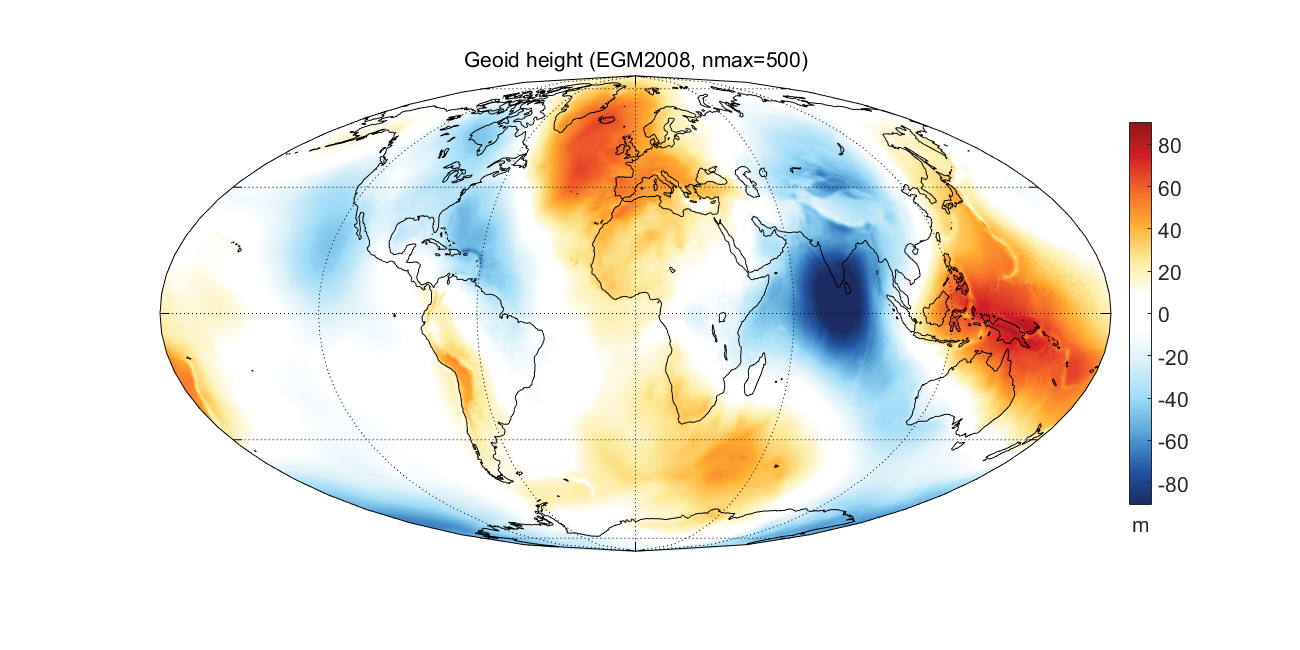
\includegraphics[width=0.8\textwidth]{obrazky/EGM2008}
    \caption{Výškový reliéf geoidu. Zdroj: \cite{Bezdek2013}}
\end{figure}

Takovýto model je poté možné použít například pomocí funkcí z Matlab Aerospace Toolbox, který vypočítá vektor gravitačního zrychlení $ a_{g} $ se správným směrem i velikostí na základě dodaný souřadnic systému WGS84. Poté pomocí rovnice \ref{eq:coriolis} můžeme vypočítat tíhové zrychlení.

\section{Rotace měření akcelerometru}
Vzhledem k tomu, že se tato práce zabývá Strapdown systémem inerciální navigace, jsou data akcelerometru vztažena k soustavě inerciální jednotky (tedy b-frame). Pro převedení dat do vztažné soustavy i-frame je potřeba rotovat vektor specific force $ \vec{f} $ maticí směrových kosínů $ \mathbf{C}_{b}^{i} $. Tato rotace by se dala popsat jako 3 po sobě jdoucí natočení o tzv. Eulerovy úhly vůči referenčním osám (např. pro tento případ i-frame). Tyto úhly označíme $ \phi $, $ \theta $ a $ \psi $ \cite{Tittertonc2004}

\begin{itemize}
\item Rotaci o úhel $ \phi $ kolem osy x přiřadíme rotační matici $ \mathbf{C}_{x} $: \cite{Tittertonc2004}
\begin{equation}
\mathbf{C}_x=\left[\begin{array}{ccc}
1 & 0 & 0 \\
0 & \cos \phi & -\sin \phi \\
0 & \sin \phi & \cos \phi
\end{array}\right]
\end{equation}

\item Rotaci o úhel $ \theta $ kolem osy y přiřadíme rotační matici $ \mathbf{C}_{y} $: \cite{Tittertonc2004}
\begin{equation}
\mathbf{C}_y=\left[\begin{array}{ccc}
\cos \theta & 0 & \sin \theta \\
0 & 1 & 0 \\
-\sin \theta & 0 & \cos \theta
\end{array}\right]
\end{equation}

\item Rotaci o úhel $ \psi $ kolem osy z přiřadíme rotační matici $ \mathbf{C}_{z} $: \cite{Tittertonc2004}
\begin{equation}
\mathbf{C}_z=\left[\begin{array}{ccc}
\cos \psi & -\sin \psi & 0 \\
\sin \psi & \cos \psi & 0 \\
0 & 0 & 1
\end{array}\right]
\end{equation} 

\end{itemize}

Součinem těchto tří matic získáme matici směrových kosinů $ \mathbf{C_{b}^{i}} $ pro převod z b-frame na i-frame: \cite{Tittertonc2004}
\begin{equation}
\mathbf{C}_{b}^{i}= (\mathbf{C}_{i}^{b})^{\mathrm{T}} = (\mathbf{C}_{x}\mathbf{C}_{y}\mathbf{C}_{z})^{\mathrm{T}} = \mathbf{C}_{z}^{\mathrm{T}}\mathbf{C}_{y}^{\mathrm{T}}\mathbf{C}_{x}^{\mathrm{T}}
\end{equation}

\begin{equation}
\mathbf{C}_{b}^{i}=
\left[\begin{array}{ccc}
\cos \theta \cos \psi & -\cos \phi \sin \psi+\sin \phi \sin \theta \cos \psi & \sin \phi \sin \psi+\cos \phi \sin \theta \cos \psi \\
\cos \theta \sin \psi & \cos \phi \cos \psi+\sin \phi \sin \theta \sin \psi & -\sin \phi \cos \psi+\cos \phi \sin \theta \sin \psi \\
-\sin \theta & \sin \phi \cos \theta & \cos \phi \cos \theta
\end{array}\right]
\end{equation}

Toto poté můžeme použít k rotaci samotného vektoru specific force $ \vec{f} $ z b-frame na i-frame

\begin{equation}
\vec{f^{i}} = \mathbf{C}_{b}^{i}\vec{f^{b}}
\end{equation}

Kombinací s rovnicí \ref{eq:aiDiffFG} získáme rovnici popisující pohyb:

\begin{equation}
\vec{a}_{i} = \left. \diff[2]{\vec{r}}{t} \right|_{i} = \vec{f^{i}} + \vec{g^{i}} = \mathbf{C}_{b}^{i}\vec{f^{b}} + \vec{g^{i}}
\end{equation}

Všechny výše popsané výpočty a děje 

\begin{figure}[h]
    \centering
    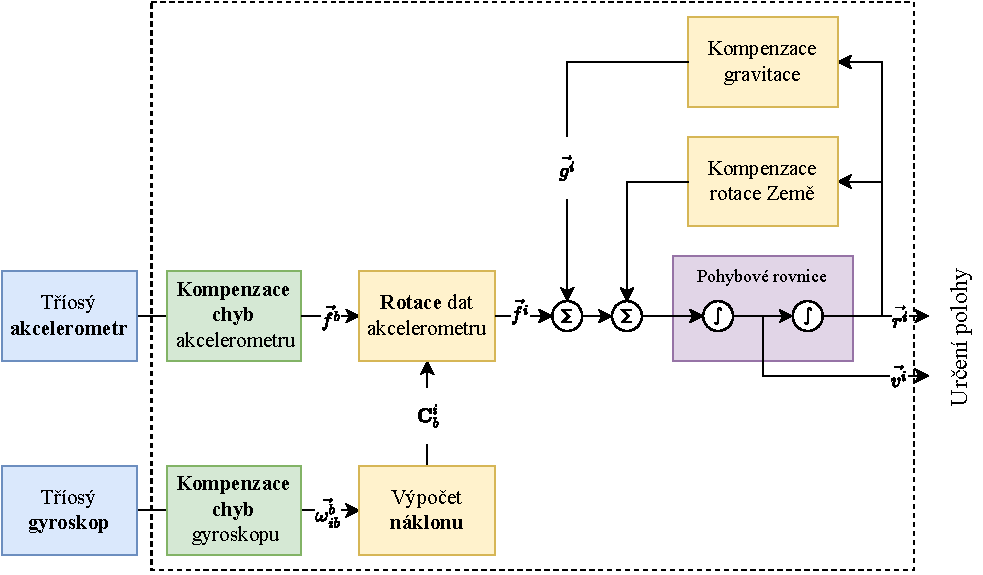
\includegraphics[width=\textwidth]{obrazky/StrapdownBlock}
    \caption{Blokové schéma algoritmu strapdown inerciální navigace, převzato z \cite{Tittertonc2004} \cite{Grewal2013} }
\end{figure}
